\documentclass[twoside]{book}

% Packages required by doxygen
\usepackage{fixltx2e}
\usepackage{calc}
\usepackage{doxygen}
\usepackage[export]{adjustbox} % also loads graphicx
\usepackage{graphicx}
\usepackage[utf8]{inputenc}
\usepackage{makeidx}
\usepackage{multicol}
\usepackage{multirow}
\PassOptionsToPackage{warn}{textcomp}
\usepackage{textcomp}
\usepackage[nointegrals]{wasysym}
\usepackage[table]{xcolor}

% Font selection
\usepackage[T1]{fontenc}
\usepackage[scaled=.90]{helvet}
\usepackage{courier}
\usepackage{amssymb}
\usepackage{sectsty}
\renewcommand{\familydefault}{\sfdefault}
\allsectionsfont{%
  \fontseries{bc}\selectfont%
  \color{darkgray}%
}
\renewcommand{\DoxyLabelFont}{%
  \fontseries{bc}\selectfont%
  \color{darkgray}%
}
\newcommand{\+}{\discretionary{\mbox{\scriptsize$\hookleftarrow$}}{}{}}

% Page & text layout
\usepackage{geometry}
\geometry{%
  a4paper,%
  top=2.5cm,%
  bottom=2.5cm,%
  left=2.5cm,%
  right=2.5cm%
}
\tolerance=750
\hfuzz=15pt
\hbadness=750
\setlength{\emergencystretch}{15pt}
\setlength{\parindent}{0cm}
\setlength{\parskip}{3ex plus 2ex minus 2ex}
\makeatletter
\renewcommand{\paragraph}{%
  \@startsection{paragraph}{4}{0ex}{-1.0ex}{1.0ex}{%
    \normalfont\normalsize\bfseries\SS@parafont%
  }%
}
\renewcommand{\subparagraph}{%
  \@startsection{subparagraph}{5}{0ex}{-1.0ex}{1.0ex}{%
    \normalfont\normalsize\bfseries\SS@subparafont%
  }%
}
\makeatother

% Headers & footers
\usepackage{fancyhdr}
\pagestyle{fancyplain}
\fancyhead[LE]{\fancyplain{}{\bfseries\thepage}}
\fancyhead[CE]{\fancyplain{}{}}
\fancyhead[RE]{\fancyplain{}{\bfseries\leftmark}}
\fancyhead[LO]{\fancyplain{}{\bfseries\rightmark}}
\fancyhead[CO]{\fancyplain{}{}}
\fancyhead[RO]{\fancyplain{}{\bfseries\thepage}}
\fancyfoot[LE]{\fancyplain{}{}}
\fancyfoot[CE]{\fancyplain{}{}}
\fancyfoot[RE]{\fancyplain{}{\bfseries\scriptsize Generated by Doxygen }}
\fancyfoot[LO]{\fancyplain{}{\bfseries\scriptsize Generated by Doxygen }}
\fancyfoot[CO]{\fancyplain{}{}}
\fancyfoot[RO]{\fancyplain{}{}}
\renewcommand{\footrulewidth}{0.4pt}
\renewcommand{\chaptermark}[1]{%
  \markboth{#1}{}%
}
\renewcommand{\sectionmark}[1]{%
  \markright{\thesection\ #1}%
}

% Indices & bibliography
\usepackage{natbib}
\usepackage[titles]{tocloft}
\setcounter{tocdepth}{3}
\setcounter{secnumdepth}{5}
\makeindex

% Hyperlinks (required, but should be loaded last)
\usepackage{ifpdf}
\ifpdf
  \usepackage[pdftex,pagebackref=true]{hyperref}
\else
  \usepackage[ps2pdf,pagebackref=true]{hyperref}
\fi
\hypersetup{%
  colorlinks=true,%
  linkcolor=blue,%
  citecolor=blue,%
  unicode%
}

% Custom commands
\newcommand{\clearemptydoublepage}{%
  \newpage{\pagestyle{empty}\cleardoublepage}%
}

\usepackage{caption}
\captionsetup{labelsep=space,justification=centering,font={bf},singlelinecheck=off,skip=4pt,position=top}

%===== C O N T E N T S =====

\usepackage{CJKutf8} 
\begin{document}
\begin{CJK}{UTF8}{gbsn} 

% Titlepage & ToC
\hypersetup{pageanchor=false,
             bookmarksnumbered=true,
             pdfencoding=unicode
            }
\pagenumbering{alph}
\begin{titlepage}
\vspace*{7cm}
\begin{center}%
{\Large tf\+\_\+test }\\
\vspace*{1cm}
{\large Generated by Doxygen 1.8.14}\\
\end{center}
\end{titlepage}
\clearemptydoublepage
\pagenumbering{roman}
\tableofcontents
\clearemptydoublepage
\pagenumbering{arabic}
\hypersetup{pageanchor=true}

%--- Begin generated contents ---
\chapter{File Index}
\section{File List}
Here is a list of all files with brief descriptions\+:\begin{DoxyCompactList}
\item\contentsline{section}{src/\hyperlink{tf__test__node_8cpp}{tf\+\_\+test\+\_\+node.\+cpp} }{\pageref{tf__test__node_8cpp}}{}
\end{DoxyCompactList}

\chapter{File Documentation}
\hypertarget{tf__test__node_8cpp}{}\section{src/tf\+\_\+test\+\_\+node.cpp File Reference}
\label{tf__test__node_8cpp}\index{src/tf\+\_\+test\+\_\+node.\+cpp@{src/tf\+\_\+test\+\_\+node.\+cpp}}
{\ttfamily \#include $<$ros/ros.\+h$>$}\newline
{\ttfamily \#include $<$tf/transform\+\_\+broadcaster.\+h$>$}\newline
{\ttfamily \#include $<$tf/transform\+\_\+listener.\+h$>$}\newline
{\ttfamily \#include $<$af\+\_\+msgs/\+Fuse\+\_\+tf.\+h$>$}\newline
Include dependency graph for tf\+\_\+test\+\_\+node.\+cpp\+:
\nopagebreak
\begin{figure}[H]
\begin{center}
\leavevmode
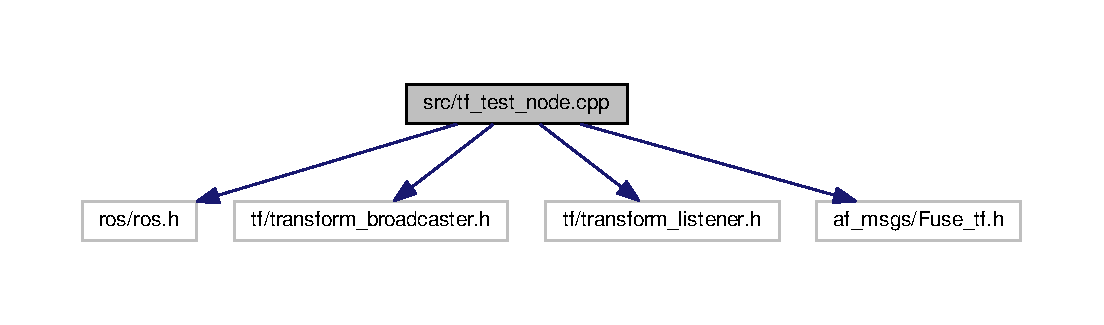
\includegraphics[width=350pt]{tf__test__node_8cpp__incl}
\end{center}
\end{figure}
\subsection*{Functions}
\begin{DoxyCompactItemize}
\item 
void \hyperlink{tf__test__node_8cpp_a82f5c406c2971a3fd11f9cc3e2740645}{tf\+Callback} (const af\+\_\+msgs\+::\+Fuse\+\_\+tf \&fuse\+\_\+tf\+\_\+msg)
\item 
int \hyperlink{tf__test__node_8cpp_a3c04138a5bfe5d72780bb7e82a18e627}{main} (int argc, char $\ast$$\ast$argv)
\end{DoxyCompactItemize}
\subsection*{Variables}
\begin{DoxyCompactItemize}
\item 
tf\+::\+Transform \hyperlink{tf__test__node_8cpp_aa6669715ce36041badf2ae04443ba28e}{map\+\_\+to\+\_\+odom\+\_\+} = tf\+::\+Transform(tf\+::create\+Quaternion\+From\+R\+PY(0, 0, 0), tf\+::\+Vector3(0.\+0, 0.\+0, 0.\+0))
\begin{DoxyCompactList}\small\item\em map-\/$>$odom全局变量 \end{DoxyCompactList}\end{DoxyCompactItemize}


\subsection{Function Documentation}
\mbox{\Hypertarget{tf__test__node_8cpp_a3c04138a5bfe5d72780bb7e82a18e627}\label{tf__test__node_8cpp_a3c04138a5bfe5d72780bb7e82a18e627}} 
\index{tf\+\_\+test\+\_\+node.\+cpp@{tf\+\_\+test\+\_\+node.\+cpp}!main@{main}}
\index{main@{main}!tf\+\_\+test\+\_\+node.\+cpp@{tf\+\_\+test\+\_\+node.\+cpp}}
\subsubsection{\texorpdfstring{main()}{main()}}
{\footnotesize\ttfamily int main (\begin{DoxyParamCaption}\item[{int}]{argc,  }\item[{char $\ast$$\ast$}]{argv }\end{DoxyParamCaption})}

main函数 \begin{DoxyVerb}将接收到的数据转换为map->odom的tf发布出来  \end{DoxyVerb}
 
\begin{DoxyCode}
32                                \{
33     ros::init(argc, argv, \textcolor{stringliteral}{"my\_tf\_broadcaster"});
34     ros::NodeHandle node;
35     ros::Subscriber sub = node.subscribe(\textcolor{stringliteral}{"/fuse/tf"}, 1, &\hyperlink{tf__test__node_8cpp_a82f5c406c2971a3fd11f9cc3e2740645}{tfCallback});
36     \textcolor{keyword}{static} tf::TransformBroadcaster br;
37     ros::Rate rate(10.0);
38     \textcolor{keywordflow}{while} (node.ok())\{
39         br.sendTransform(tf::StampedTransform (\hyperlink{tf__test__node_8cpp_aa6669715ce36041badf2ae04443ba28e}{map\_to\_odom\_}, ros::Time::now(), \textcolor{stringliteral}{"map"}, \textcolor{stringliteral}{"odom"}));
40         ros::spinOnce();
41         rate.sleep();
42     \}
43     \textcolor{keywordflow}{return} 0;
44 \};
\end{DoxyCode}
\mbox{\Hypertarget{tf__test__node_8cpp_a82f5c406c2971a3fd11f9cc3e2740645}\label{tf__test__node_8cpp_a82f5c406c2971a3fd11f9cc3e2740645}} 
\index{tf\+\_\+test\+\_\+node.\+cpp@{tf\+\_\+test\+\_\+node.\+cpp}!tf\+Callback@{tf\+Callback}}
\index{tf\+Callback@{tf\+Callback}!tf\+\_\+test\+\_\+node.\+cpp@{tf\+\_\+test\+\_\+node.\+cpp}}
\subsubsection{\texorpdfstring{tf\+Callback()}{tfCallback()}}
{\footnotesize\ttfamily void tf\+Callback (\begin{DoxyParamCaption}\item[{const af\+\_\+msgs\+::\+Fuse\+\_\+tf \&}]{fuse\+\_\+tf\+\_\+msg }\end{DoxyParamCaption})}

fuse/tf 回调函数 \begin{DoxyVerb}topic /fuse/tf 回调过程中调用,并且将fuse_tf_msg分解为map->base和odom->base两组数据,转换为map->odom并传递到main函数循环中
\end{DoxyVerb}
 
\begin{DoxyParams}{Parameters}
{\em fuse\+\_\+tf\+\_\+msg} & 自定义\+Fuse\+\_\+tf格式数据 \\
\hline
\end{DoxyParams}
\begin{DoxyReturn}{Returns}
无返回值 
\end{DoxyReturn}
\begin{DoxyNote}{Note}
临时解决方案 
\end{DoxyNote}

\begin{DoxyCode}
18                                                   \{
19     tf::Transform laser\_to\_map = tf::Transform(tf::createQuaternionFromRPY(0, 0, fuse\_tf\_msg.map\_theta), 
      tf::Vector3(fuse\_tf\_msg.map\_x, fuse\_tf\_msg.map\_y, 0.0)).inverse();
20     tf::Transform odom\_to\_laser = tf::Transform(tf::createQuaternionFromRPY(0, 0, fuse\_tf\_msg.odom\_theta), 
      tf::Vector3(fuse\_tf\_msg.odom\_x, fuse\_tf\_msg.odom\_y, 0.0));
21     
22     \hyperlink{tf__test__node_8cpp_aa6669715ce36041badf2ae04443ba28e}{map\_to\_odom\_} = (odom\_to\_laser * laser\_to\_map).inverse();
23     \textcolor{comment}{//map\_to\_odom\_ = tf::Transform(tf::createQuaternionFromRPY(0, 0, 0), tf::Vector3(0.0, 0.0, 0.0));}
24     ROS\_INFO(\textcolor{stringliteral}{"x=%f,y=%f"},\hyperlink{tf__test__node_8cpp_aa6669715ce36041badf2ae04443ba28e}{map\_to\_odom\_}.getOrigin().getX(),
      \hyperlink{tf__test__node_8cpp_aa6669715ce36041badf2ae04443ba28e}{map\_to\_odom\_}.getOrigin().getY());
25       ROS\_INFO(\textcolor{stringliteral}{"processing tf"});
26 \}
\end{DoxyCode}


\subsection{Variable Documentation}
\mbox{\Hypertarget{tf__test__node_8cpp_aa6669715ce36041badf2ae04443ba28e}\label{tf__test__node_8cpp_aa6669715ce36041badf2ae04443ba28e}} 
\index{tf\+\_\+test\+\_\+node.\+cpp@{tf\+\_\+test\+\_\+node.\+cpp}!map\+\_\+to\+\_\+odom\+\_\+@{map\+\_\+to\+\_\+odom\+\_\+}}
\index{map\+\_\+to\+\_\+odom\+\_\+@{map\+\_\+to\+\_\+odom\+\_\+}!tf\+\_\+test\+\_\+node.\+cpp@{tf\+\_\+test\+\_\+node.\+cpp}}
\subsubsection{\texorpdfstring{map\+\_\+to\+\_\+odom\+\_\+}{map\_to\_odom\_}}
{\footnotesize\ttfamily tf\+::\+Transform map\+\_\+to\+\_\+odom\+\_\+ = tf\+::\+Transform(tf\+::create\+Quaternion\+From\+R\+PY(0, 0, 0), tf\+::\+Vector3(0.\+0, 0.\+0, 0.\+0))}



map-\/$>$odom全局变量 


%--- End generated contents ---

% Index
\backmatter
\newpage
\phantomsection
\clearemptydoublepage
\addcontentsline{toc}{chapter}{Index}
\printindex

\end{CJK} 
\end{document}
